\documentclass[a4paper]{article}
\usepackage[T1]{fontenc}
\usepackage[utf8]{inputenc}%\usepackage[latin1]{inputenc}
\DeclareUnicodeCharacter{0301}{\'{e}}
\usepackage{graphicx}
\usepackage{hyperref}
\hypersetup{
  setpagesize  = false,
  colorlinks   = true,    % Colours links instead of ugly boxes
  urlcolor     = blue,    % Colour for external hyperlinks
  linkcolor    = black,   % Colour of internal links
  citecolor    = black    % Colour of citations
}
\urlstyle{same} 

\usepackage{authblk}
\usepackage{geometry}
\usepackage{setspace}
\usepackage{verbatim}
\usepackage[utf8]{inputenc}
\usepackage{amsmath}
\usepackage{amssymb}
\usepackage{gensymb}
\usepackage{verbatim} % env for block comment 
\usepackage{ragged2e} % para usar flusleft
\usepackage{minted}
\usemintedstyle{tango}
\usepackage{amsfonts}
\usepackage{cancel}
\usepackage{graphicx}
\graphicspath{ {./images/} }



\setcounter{page}{1} % página inicial do artigo
%==========================================================================
% Margens e tamanho da página
%==========================================================================
\setlength{\paperwidth}{19cm}\setlength{\paperheight}{29cm}
\setlength{\textwidth}{16cm}\setlength{\textheight}{23cm}
\setlength{\oddsidemargin}{2cm}
\setlength{\headheight}{\baselineskip}
\setlength{\topmargin}{3cm}
%\setlength{\headsep}{2cm}\addtolength{\headsep}{-\headheight}
\setlength{\footskip}{2cm}\addtolength{\footskip}{.5\baselineskip}
\addtolength{\topmargin}{-1in}
\addtolength{\oddsidemargin}{-1in}
\setlength{\evensidemargin}{\oddsidemargin}
%==========================================================================
% Definições diversas
%==========================================================================
\setlength{\parindent}{1cm}
\newcommand{\abstractinenglishname}{Abstract}
\newcommand{\keywordsportugues}{Palavras-chave}
\newcommand{\keywordsenglishname}{Keywords}



%==========================================================================
% Resumo (abstract) e Abstract (englishabstract)
%==========================================================================
\renewenvironment{abstract}{%
        \begin{center}
	\begin{minipage}{14cm}
	{\textbf{\abstractname:}}
}{
        \end{minipage}
	\end{center}
}
\newenvironment{abstractinenglish}{
        \def\abstractname{\abstractinenglishname}
	\begin{abstract}
}{
        \end{abstract}
}
%==========================================================================
% Palavras-chave (keywords) e Keywords (keywordsenglish)
%==========================================================================
\newenvironment{keywords}{
        \def\abstractname{\emph{\keywordsportugues}}
	\begin{abstract}
}{
        \end{abstract}
}
\newenvironment{keywordsenglish}{
        \def\abstractname{\emph{\keywordsenglishname}}
	\begin{abstract}
}{
        \end{abstract}
}

%==========================================================================
% Artigo
%==========================================================================

\title {Heart Disease Prediction}
\author{Ian Chuang, Joshua Winerman, Arjun Kahlon, Darrel Chiou, Nathan Liu, Ho-Chih Ma, Shaivya Padia}
\affil{UC Davis ECS 171 Group Project}
\date{}

\usepackage{fancyhdr}
\fancyhf{}

%==========================================================================
% Não editar o cabeçalho
%==========================================================================

%==========================================================================
% Não editar o cabeçalho
%==========================================================================
\fancyhead[R]{\thepage}
\pagestyle{fancy}

\begin{document}

\maketitle
\vspace{6pt}


\section{Introduction and Background}

Healthcare today works hard to both predict and remedy diseases worldwide. Amongst the challenges faced, ischaemic heart disease continues to be the number one cause of death globally \cite{death}. In a world where so many people have pre-existing conditions, and nearly every choice made can negatively impact one’s health, it is crucial to be aware of your own susceptibility. Lifestyle choices such as smoking, alcohol consumption, and sleep time; health conditions such as diabetes, stroke, and asthma; and personal factors such as race, age, and sex can contribute to predicting the likelihood of heart disease \cite{mayoclinic}.

The progress of technology changes the way diseases are detected and treated every day. With the growing advances in the field of machine learning, the healthcare industry can be revolutionized with the help of different machine learning models which could help in making diagnoses faster and more accurately than ever. Heart diseases can be treated in most cases if diagnosed early on, time being the essence. However, in many cases, they are left undetected, especially in certain communities and women \cite{minorities}. As women experience very different symptoms compared to men, they sometimes do not know if they are having a heart attack and hence cannot ask for the help that they need \cite{women}.  

With the help of an accurate machine learning model, people can be made more aware and it can be used in many different ways, for example: 


\begin{itemize}
   \item Self Checking:
   \begin{itemize}
     \item People can put in values for the different attributes in a model, and that would predict their chances of having heart disease. If they have a higher chance they could make lifestyle changes as well as get routine checkups with their doctor so that it can be caught early on before it becomes serious.
   \end{itemize}
   \item Aiding Doctors:
   \begin{itemize}
     \item These sorts of machine learning models can be used by doctors when they take their patient’s histories. If the model indicates a higher likelihood of heart disease then the doctor can make certain recommendations as well as be on the lookout. 
   \end{itemize}
 \end{itemize}

This paper aims to develop an accurate machine learning model that could be used in these applications. We perform data analysis on the Personal Key Indicators of Heart Disease dataset, which is a 2020 annual CDC survey of the health of 400,000 adults \cite{dataset}. We explore what attributes such as BMI, smoking, drinking alcohol, etc are highly correlated with heart disease. We then develop a variety of models to predict whether someone is susceptible to getting heart disease based on various factors. We will use logistic regression, Naive Bayes, decision trees, linear support vector machines, and multilayer neural networks and see which model performs best. 


\section{Literature Review}

This is not the first time that people have made use of machine learning to predict the probability of heart failure. In several previous cases, researchers have used a wide variety of models and tools provided by machine learning to help identify heart disease in an individual. In this section, we will review and analyze a previous case where machine learning was used to combat heart failure.

This study, conducted by Computational Intelligence and Neuroscience, used machine learning to predict the occurrence of cardiovascular failure \cite{review}. Here, the researchers used two unique datasets. The first dataset was the Hungarian dataset, created by the Hungarian Institute of Cardiology in Budapest with 294 individual instances. The second dataset was the Statlog (heart) dataset. Combined, their database contained 76 different attributes. They performed data analysis to extract the most important features and decrease complexity while maintaining performance, leaving them with 14 total attributes to be used in their experiments. Then after further data preprocessing and filtering of the raw data, to fix values and reduce overall noise, the study implemented several different machine learning methods to analyze both datasets, which consisted of REP Tree, M5P, Linear Regression, and Random Tree for the Hungarian dataset and Naive Bayes, J48, Random Tree, and JRIP for the Statlog (heart) dataset. They then measured the Mean Absolute Error, Root Mean Squared Error, accuracy, and time to help identify the best prediction model. 

From their results, it could be seen that Random Tree was the most accurate and efficient model when applied to each of the datasets. For the Hungarian dataset, Random Tree obtained the highest accuracy at 99.81\% and the second-lowest execution time at 0.02 secs with an MAE similar to the other models at .2838, though its RMSE was greater than the other three models at .5328. Linear Regression also performed well when applied to the dataset with the smallest RMSE at .371, smallest execution time at 0.01 secs, and moderate MAE of .2978, though it lacked accuracy with the smallest percent of 74.32\%. For the Statlog (heart) database, Random Tree also stood out with an MSE of .0011, RMSE of .0231, accuracy of 100\%, and execution time of .01 secs, which were all either the most ideal or tied for the most ideal values in their respective classes. The Naive Bayes model, though, also performed well when applied to the Statlog (heart) dataset as it had an identical performance to Random Tree when used.   

This paper will look to further expand on this study, by not only developing similar models like Naive Bayes and Decision Trees but also introducing tools like Logistic Regression and Neural Networks. 


\section{Dataset Description and Exploratory Data Analysis}

The dataset this paper will use is the Personal Key Indicators of Heart Disease dataset. This dataset is a survey conducted by the CDC on the health status of around 400,000 US adults \cite{dataset}. We chose to use this dataset since it includes many common and easily measurable attributes related to general health. This fits our purposes since anyone could easily fill out a form of their health history and get quick results from any model we make.

\subsection{Dataset Attribute Information}

In the dataset, Heart Disease is the target column that we want to predict. Columns 2 - 5 are numerical attributes, while columns 6 - 18 are categorical attributes.

\begin{enumerate}
\item Heart Disease: A Yes/No value that reports whether the individual has coronary heart disease or myocardial infarction. This can be converted into a binary value.
\item BMI: Stands for body mass index, it is a numerical value. BMI is calculated by an individual's weight in kilograms divided by height in meters squared.
\item Physical Health: This is a numerical attribute that is determined by how many of the past 30 days an individual has had physical illness or injury. 
\item Mental Health: This is a numerical attribute that is determined by how many of the past 30 days an individual had bad mental health.
\item Sleep Time: A numerical attribute that is determined by how many hours of sleep they typically get within 24 hours.
\item Smoking: A Yes/No value that is determined by whether an individual has smoked at least 100 cigarettes (5 packs) in their lifetime. This can be converted into a binary value.
\item Alcohol Drinking: A Yes/No value that is determined by whether an individual is a heavy drinker (14 drinks a week for men and 7 drinks a week for women). This can be converted to a binary value.
\item Stroke: A Yes/No value that is determined by whether an individual has had a stroke. This can be converted into a binary value.
\item Difficulty Walking: A Yes/No value that is determined by whether an individual has difficulty walking. This can be converted into a binary value.
\item Sex: A categorical variable that distinguishes males and females. This can be converted into a binary value.
\item Physical Activity: A Yes/No value that is determined by whether an individual has done physical exercise during the past 30 days. This can be converted into a binary value.
\item Asthma: A Yes/No value that is determined by whether an individual has asthma. This can be converted into a binary value.
\item Kidney Disease: A Yes/No value that is determined by whether an individual has kidney disease (not including kidney stones, bladder infection, or incontinence). This can be converted into a binary value.
\item Skin Cancer: A Yes/No value that is determined by whether an individual has skin cancer. This can be converted into a binary value.
\item Age Category: A categorical variable that determines the age range of an individual. There are 14 total categories: 17 or younger, 18-24, 25-29, 30-34, 35-39, 40-44, 45-49, 50-54, 55-59, 60-64, 65-69, 70-74, 75-79, 80 or older
\item Race: A categorical variable that is determined by the race/ethnicity of an individual. There are total categories: White, Hispanic, Black, Asian, American Indian/Alaskan Native, and Other.
\item Diabetic: A categorical variable that is determined whether an individual has had diabetes or not. Includes pregnancy diabetes.
\item General Health: A categorical variable that classifies their general health into the following groups: Excellent, Very good, Good, Fair, Poor.
 \end{enumerate}
 
 \subsection{Exploratory Data Analysis}

We then plotted numerical attributes as kernel density estimation curves and categorical attributes as histograms, separating people with and without heart disease, to get an idea of the distributions of the attributes.

\begin{figure}[H]
    \centering
    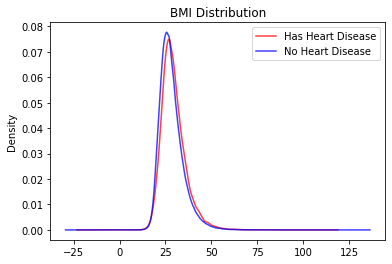
\includegraphics[width=7cm]{images/bmi.png}
    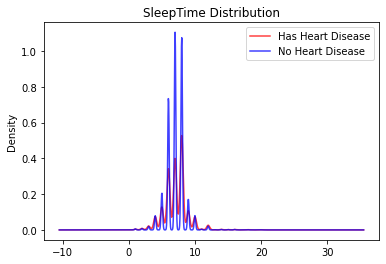
\includegraphics[width=7cm]{images/sleeptime.png}
\end{figure}

In terms of numerical variables, ‘BMI’ and ‘Sleep Time’ seem to have a relatively normal distribution. When we distinguish between those with and without heart disease for BMI, there is very little difference between the two groups. This suggests that BMI does not have that high of an impact on heart disease. This is similar to sleep time, where the distribution of sleep time for individuals with and without heart disease are both normal, suggesting that sleep time has little impact on heart disease.

\begin{figure}[H]
    \centering
    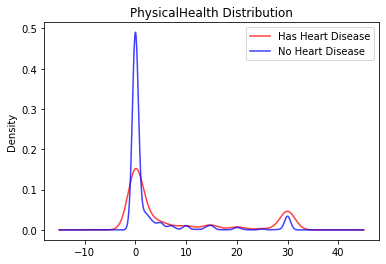
\includegraphics[width=7cm]{images/physicalhealth.png}
    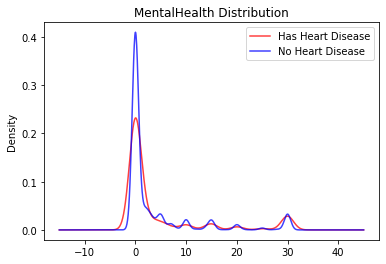
\includegraphics[width=7cm]{images/mentalhealth.png}
\end{figure}

On the other hand, the ‘PhysicalHealth’ and ‘MentalHealth’ distributions seem to be more extreme around the minimum (0 days) and maximum (30 days), with an emphasis on the minimum (better health). From this, we can assume that most individuals were on the healthier side of the spectrum. After distinguishing between those with and without heart disease, however, it is evident that those on the maximum side experience heart disease more, while those on the minimum side experience heart disease less. Thus, we can conclude that mental health and physical health are key factors that determine whether someone will get heart disease.

\begin{figure}[H]
    \centering
    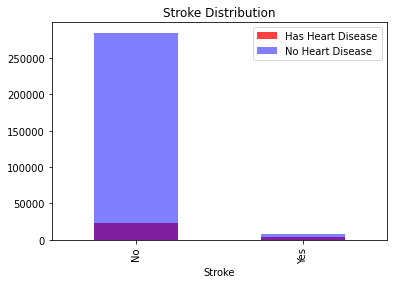
\includegraphics[width=7cm]{images/stroke.png}
    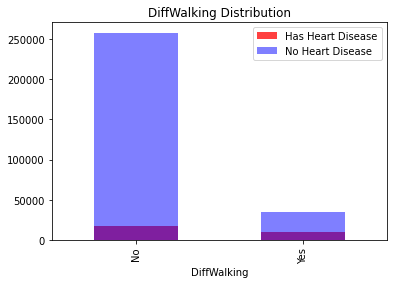
\includegraphics[width=7cm]{images/difficultywalking.png}
\end{figure}

For the categorical variables like ‘Smoking’, ‘AlcoholDrinking’, ‘Stroke’, ‘DiffWalking’, ‘Asthma’, ‘KidneyDisease’, ‘SkinCancer’, and ‘Diabetic’, the majority of individuals responded with ‘No’. From this, we can conclude that the population is relatively healthy. However, out of those who responded with ‘Yes’ for these attributes, they had a much higher chance of having heart disease than those who responded with ‘No’. Thus, we can conclude that there is a correlation between heart disease and smoking, alcohol drinking, stroke, etc.

\begin{figure}[H]
    \centering
    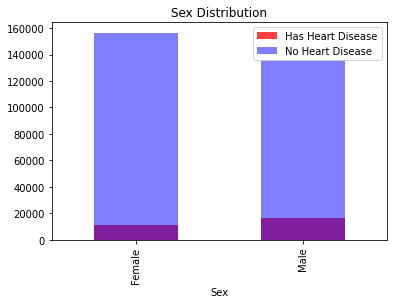
\includegraphics[width=7cm]{images/sex.png}
    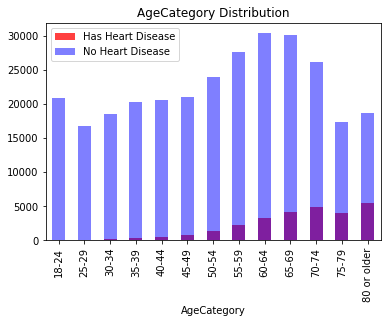
\includegraphics[width=7cm]{images/agecategory.png}
\end{figure}

For the ‘Sex’ variable, there were a relatively equal number of males and females. After creating a bar plot that distinguished the ‘Yes’s’ and ‘No’s’ within each category, it seems that males have a higher chance of having heart disease than females. There is a similar trend with the ‘AgeCategory’ variable, where there is a roughly normal distribution in terms of the age group of the population. However, heart disease seems to be more prevalent in older individuals (aged 50+ at 5\%+) than younger individuals (below age 49).

\begin{figure}[H]
    \centering
    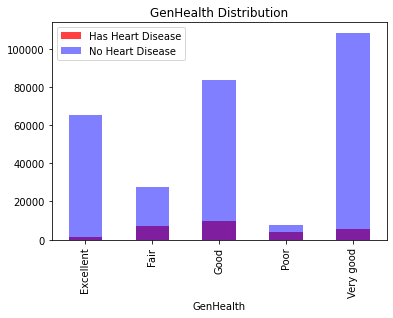
\includegraphics[width=7cm]{images/genhealth.png}
\end{figure}

In terms of the ‘GenHealth’ Distribution, Those with ‘Poor’ health have a significantly higher chance of getting heart disease (34.10\%) than those with ‘Excellent’ health (2.24\%). This suggests a correlation between the general health of an individual and whether or not they will get heart disease.

\begin{figure}[H]
    \centering
    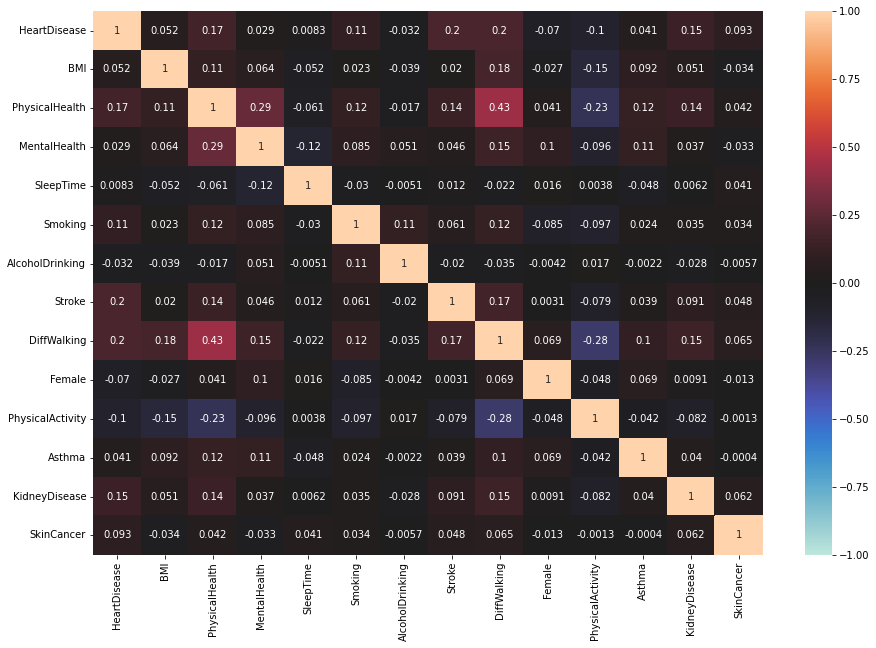
\includegraphics[width=14cm]{images/correlationmatrix.png}
\end{figure}

We also created a covariance matrix between all binary and numerical attributes. Based on the covariance matrix, Heart Disease is positively correlated with Physical Health, Stroke, Kidney Disease, Smoking, and Difficulty Walking. In terms of other correlations between the other independent variables, Physical health, Physical activity, and Difficulty walking seem to have a high correlation with many of the other variables (Stroke, BMI, Mental Health, etc). 

We did not find much bias in the data because there weren’t any NA values. Additionally, there wasn’t any data that doesn’t make sense


\section{Proposed Methodology}

We must first perform data pre-processing to clean and prepare our dataset. We make sure there are no mislabeled attributes, remove any data which have missing data, and convert binary categorical data to ones and zeros. We then apply min-max normalization on any numerical attributes in our dataset, transforming all numerical values to be between 0 and 1. This helps our model treat each numerical attribute equally, without creating bias between attributes. Finally, we perform one-hot encoding on any categorical attributes so that we can easily feed them into our models. On a separate dataset, we perform ordinal encoding instead for our Naive Bayes model.
We then split 90\% of our dataset into a training set and 10\% into a testing set. We have a test set so that we have a reliable way of measuring the performance of our models without introducing any biases from our train set. We split the one-hot encoded and ordinal encoded datasets individually. 
	
We used a variety of different models to gauge which one performs best. The first model we implemented is logistic regression since it is commonly used to model binary classification. Logistic regression uses a linear combination of the input and a set of weights and the sigmoid activation function to perform gradient descent, maximizing the likelihood of a correct prediction. The next model we used was the decision tree classifier. Decision trees are a non-parametric model that uses a tree-like structure to make inferences about the data. We also tried a linear support vector machine (SVM) which uses a hyperplane to separate the data. Another model we use is the Naive Bayes model. For Naive Bayes, there are two different models, Categorical Naive Bayes and Gaussian Naive Bayes. We will perform categorical Naive Bayes on our ordinal encoded dataset, only using categorical attributes. Gaussian Naive Bayes will use only numerical attributes. For all these models, we used the scikit-learn library in Python.

Finally, the last two models we tried are two different versions of a Multilayer Neural Network. We first create a baseline neural network model to measure how well a standard neural network would perform on the dataset. This baseline model will have two hidden layers, 32 nodes each, with Relu activation functions, and a final output layer of 1 node with a sigmoid activation function. We chose to use Relu for the hidden layers to avoid the vanishing gradient problem and sigmoid for the final layer since the output will have a probability from 0 to 1. Other hyperparameters will include a 10\% validation split, batch size of 32, 5 epochs, a learning rate of 0.01, and using the Adam optimizer. We chose to only use 5 epochs because we noticed in training that the model learns very quickly but plateaus after only 1 to 2 epochs. We also used the Adam optimizer since it is well regarded as a top-performing optimizer that speeds up learning.
The next step we tried to improve and evaluate our neural network’s performance is K-Fold Cross Validation. K-Fold Cross Validation helps see if there is any bias in our data. By resampling our data 5 folds we test if our model can handle learning to different samples of our data.

Finally, we tried implementing Grid Search for hyperparameter tuning. Grid Search tries different variations of hyperparameters to see which set of hyperparameters makes the model perform best. For our Grid Search, we have six different hyperparameters to vary: the number of hidden layers, the number of nodes for each hidden layer, the learning rate, whether to use dropout in our hidden layers, whether to use L2 regularization in our hidden layers, and the number of epochs. We chose these hyperparameters and values through our best judgment of potential parameters that could improve accuracy. 

Once we perform all these steps, we will pick the best model from grid search and use it as our “optimized” neural network. We used the Keras library to implement all the neural networks.

For evaluating all the different models we are creating, we will report the overall accuracy, precision, recall, and f1-score for each model. We will also create a confusion matrix to count false positives, false negatives, true positives, and true negatives. From these evaluation metrics, we can decide the best model to use for our demonstrations. 


\section*{Experimental Results}

Before we discuss the results of each model, we first show the results from K-Fold Cross Validation and Grid Search that we used to construct our optimized Neural Network.

\subsection{5-Fold Cross Validation}

\texttt{Fold 1 - MSE: 0.08322519113807282; Acc: 0.9167748088619272\% \\
Fold 2 - MSE: 0.08571115871104927; Acc: 0.9142888412889507\% \\
Fold 3 - MSE: 0.08313138104097938; Acc: 0.9168686189590206\% \\
Fold 4 - MSE: 0.0840382119795494; Acc: 0.9159617880204506\% \\
Fold 5 - MSE: 0.08607076408324082; Acc: 0.9139292359167591\% \\
Average - MSE: 0.08443534139057834; Acc: 0.9155646586094216\%} \\

Across all five different folds of K-fold Cross Validation with k=5, the baseline model accuracy was around 91.5\% and did not vary very much. Since the model performance does not vary significantly across different resamplings of the dataset, we can conclude that the baseline neural network can generalize well to the data. Thus, no further optimizations are needed for resampling the dataset. 

\subsection{Grid Search}

After running Grid Search, the Neural Network model with the best performance had only one hidden layer with 32 nodes, used dropout, had a smaller learning rate of 0.001, didn’t use L2 regularization, and ran for three epochs. Despite using only 1 hidden layer, the model outperformed those that used up to three hidden layers. We infer that this is due to the simplicity of the dataset since a more complex model might overfit whereas a simpler model will generalize better. Another interesting point is that a smaller learning rate is better. This is most likely because learning the dataset doesn’t take very long, so a smaller learning rate can still reach the minimum loss quickly while being more precise. Dropout seemed to help performance whereas L2 regularization hurt performance. It is unclear to us why this occurred and requires further research.

\subsection{Creating an Optimized Neural Net}

Using the best model from grid search, we train it again individually on the dataset for eight epochs. We decided to train for more epochs to see if we can further reduce the loss. We stop training once the loss has plateaued to avoid overfitting.

\begin{figure}[H]
    \centering
    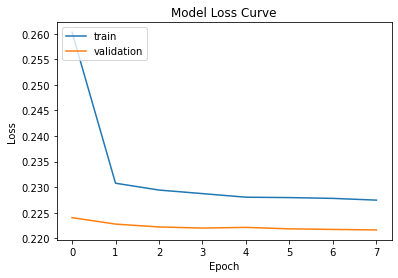
\includegraphics[width=10cm]{images/modellosscurve.png}
\end{figure}

\subsection{Model Performance on Testing Set}

\begin{figure}[H]
    \centering
    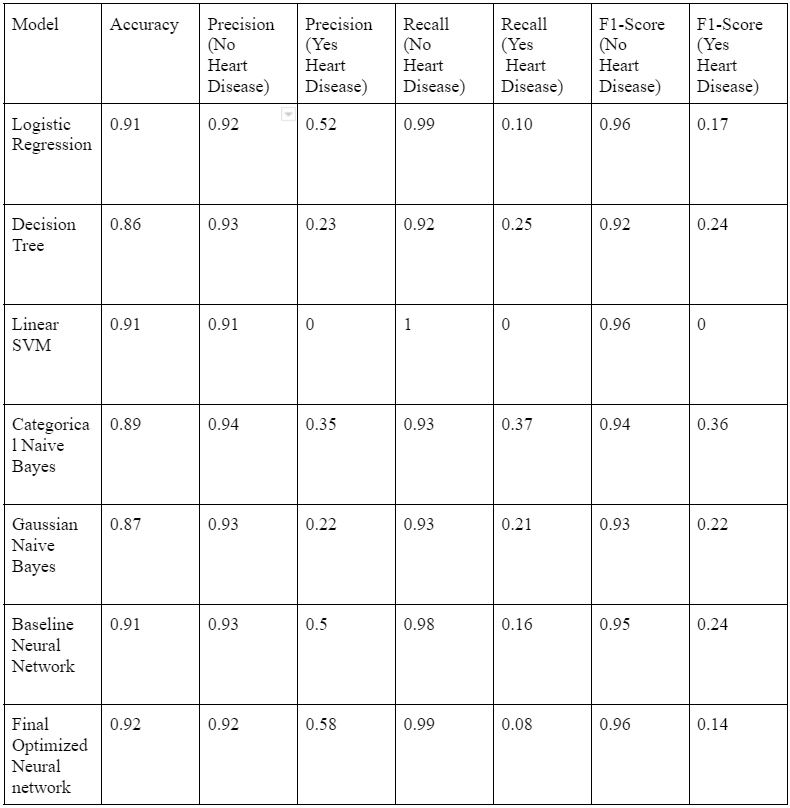
\includegraphics[width=12cm]{images/classificationreport.png}
\end{figure}

\subsection{Confusion Matrix of Each Model on Test Set}

\begin{figure}[H]
    \centering
    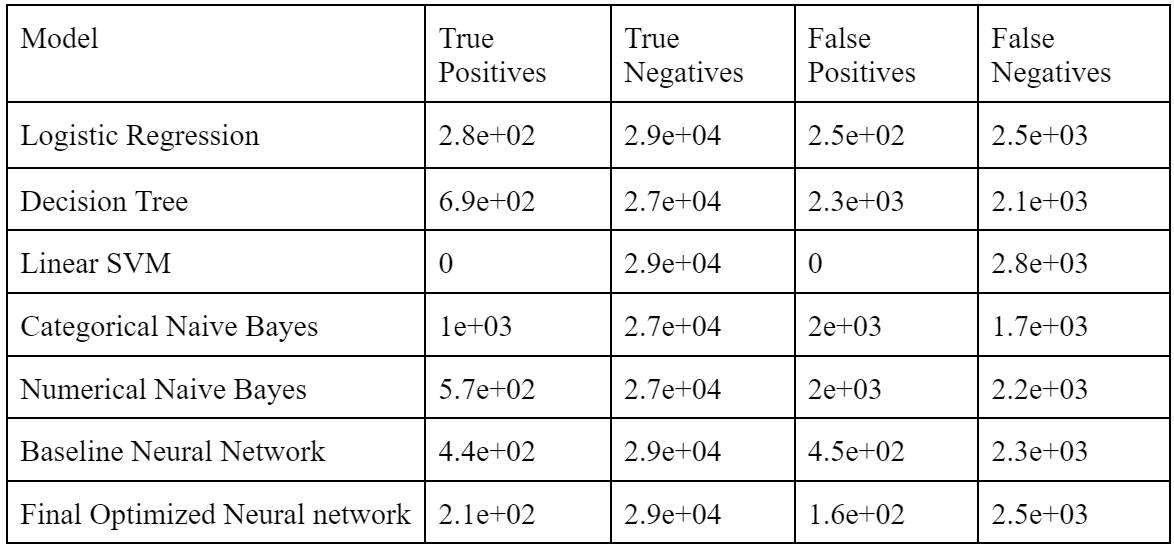
\includegraphics[width=12cm]{images/confusionmatrix.png}
\end{figure}

\subsection{Logistic Regression}

The Logistic Regression model performs fairly well in comparison to the other models. It has the best accuracy out of all models that aren’t Neural Networks. However, its precision, recall, and f1-score for people with heart disease are significantly lower than for people without heart disease. This means that the model is inaccurately classifying people who have heart disease, but is accurate for people without heart disease. Logistic Regression has one of the lowest recall for people with heart disease, just 10\%, meaning it is only recognizing 10\% of the people with heart disease.

\subsection{Decision Tree}

The Decision Tree model has the worst overall accuracy out of all the models. Despite this, the f1 score and recall for people with heart disease in the decision tree model are higher than that of Logistic Regression. This means that the Decision Tree is more likely to classify a person as having heart disease than logistic regression. However, this also lowers its precision and makes the decision tree model have the most false positives out of all other models. The decision tree model was likely inaccurate due to overfitting, which commonly occurs in Decision Trees.

\subsection{Linear SVM}

While the Linear SVM has higher overall accuracy than the Decision Tree model, it is by far the worst-performing model. This is because the Linear SVM had zero true positives and zero false positives, meaning it classified every person as not having heart disease. Since 91.4\% of people in the dataset do not have heart disease, the accuracy is naturally high, but the model is useless as a classifier. We believe Linear SVM failed because a single hyperplane is not enough to model the data.


\subsection{Categorical Naive Bayes}

While the overall accuracy of Categorical Naive Bayes is not too high, the f1-score and recall for people with heart disease are the highest out of all other models. Its precision for detecting if a person has heart disease is also relatively high and it has the highest number of true positives. This means the model classifies more people as having heart disease while still having decent precision. However, the number of false positives is still very large in comparison to the Neural Network and Logistic Regression models.

\subsection{Numerical Naive Bayes}

Numerical Naive Bayes has similar results to the Decision Tree model overall. It has low accuracy, but still has minimal improvements in recall and f1-score for people who have heart disease compared to logistic regression. This poor performance is most likely due to the model not having enough data as there are only four numerical attributes.


\subsection{Baseline Neural Network}

The baseline Neural Network has similar accuracy to Logistic Regression but has a higher recall and f1-score for people with heart disease. The precision is still comparable to logistic regression, but the model has almost twice the amount of false positives. This model identifies more people who have heart disease, at the risk of having more false positives.  
	
\subsection{Final Optimized Neural Network}

The final optimized Neural Network has the highest overall accuracy out of all the models. However, other than linear SVM, the model has the lowest recall and f1-score for people who have heart disease out of all models. This is a sign that the optimized neural network is not very reactive when predicting when someone has heart disease and is much more likely to lean towards a person not having heart disease. This is shown by the model having the lowest number of false positives (other than linear SVM) and the highest precision for people who have heart disease.
	
\subsection{Summary of Experimental Results}

The optimized Neural Network was the most accurate model. This is because this neural network was specially optimized for this dataset using grid search. It has features like a small learning rate and using dropout that make it robust.

From the results of the different models, there is a very clear trade-off between the number of false positives and the recall rate for people who have heart disease. If a model is more reactive to predicting people as having heart disease, you risk having more false positives. If the model is less reactive, you won’t be able to identify as many people with heart disease.

The recommended model to use depends on the situation and how sensitive you want the model to be. For example, in self-checking, it is ideal to minimize the number of false positives so the model does not alarm too many users. The optimized Neural Network is the best model for this application. However, in aiding doctors with an initial diagnosis, having a high recall and being more sensitive to detecting heart disease is more important so that more people who do have heart disease will be alerted and can get a further diagnosis by their doctor. In this example, the baseline Neural Network would be a better choice. 

Another interesting result is that no matter how long you train a model on the dataset, the training accuracy peaks at around 92\%. This is a sign that more attributes and indicators are needed in the dataset to improve accuracy and give a more proper diagnosis of heart disease. 

\section*{Conclusion and Discussion}

Cardiovascular diseases cause a majority of deaths in the world and can be caused by multiple factors. In this report, we analyzed the significance of patient lifestyle choices such as smoking, alcohol consumption, and sleep time; as well as health conditions such as diabetes, strokes, and asthma; and personal factors such as race, age, and sex. To do so, machine learning models including logistic regression, decision tree classifier, linear SVM, Naive Bayes, and Neural Networks were utilized.

To determine the validity of our models, we use mean squared error, classification reports, and confusion matrices. Through these metrics, it was determined that the best model to use was the optimized Neural Network, which had the best possible combination of true positive and false positive cases. While the false positive rate is low for the optimized Neural Network, this results in a tradeoff of a higher false negative rate which indicates that the model is more conservative and will more likely predict that a patient does not have heart disease.

To improve upon the models described in this paper, certain things can be done. Two of which are to have more indicators besides the ones already used. Another method would be to have an even larger proportion of people in the data set with heart disease to balance out the training set.

While this still has the potential to be further optimized, there are a lot of practical applications for a model that can predict heart disease. Many lives could be saved with preventive healthcare, and with further improvement, there are many usages for a machine learning model capable of predicting heart disease.


\begin{thebibliography}{9}
\bibitem{dataset}
https://www.kaggle.com/datasets/kamilpytlak/personal-key-indicators-of-heart-disease/code

\bibitem{women}
“Heart Disease in Women: Unsuspected? Overlooked? Ignored? - Mayo Clinic Press.” Mayo Clinic, Mayo Foundation for Medical Education and Research, 14 Feb. 2022, https://mcpress.mayoclinic.org/women-health/part-1-heart-disease-in-women-unsuspected-overlooked-ignored/. 

\bibitem{mayoclinic}
“Heart Disease.” Mayo Clinic, Mayo Foundation for Medical Education and Research, 9 Feb. 2021, http://www.mayoclinic.org/diseases-conditions/heart-disease/diagnosis-treatment/drc-20353124. 

\bibitem{minorities}
Leigh, J Adam, et al. “Ethnic Minorities and Coronary Heart Disease: An Update and Future Directions.” Current Atherosclerosis Reports, U.S. National Library of Medicine, Feb. 2016, http://www.ncbi.nlm.nih.gov/pmc/articles/PMC4828242/. 

\bibitem{death}
O'Riordan, Michael. “Ischemic Heart Disease the Leading Cause of Death Globally.” TCTMD.com, TCTMD.com, 13 May 2021, http://www.tctmd.com/news/ischemic-heart-disease-leading-cause-death-globally. 

\bibitem{review}
Nadakinamani, Rajkumar Gangappa, et al. “Clinical Data Analysis for Prediction of Cardiovascular Disease Using Machine Learning Techniques.” Computational Intelligence and Neuroscience, Hindawi, 11 Jan. 2022, https://www.ncbi.nlm.nih.gov/pmc/articles/PMC8767405/\#B25. 

\end{thebibliography}

\end{document} 